\documentclass{report}

% ----------------------------------------------------------------------------
% Preamble
% ----------------------------------------------------------------------------

% These are some lazy packages to get a good looking page layout
\usepackage{fullpage}
\usepackage[parfill]{parskip}

\usepackage{setspace}
\onehalfspacing

% A package to include graphics files (jpg, png, eps, pdf etc...)
%\usepackage{epstopdf}
\usepackage{graphicx}

% Some basic packages that are almost standad
\usepackage{amssymb}
\usepackage{amsmath}

% Package to be able to draw tikz images
\usepackage{tikz}
\usetikzlibrary{calc}

% Package to get hyperrlinks
\usepackage{hyperref}

% Package to be able to compile standalone tikz packages
\usepackage{standalone}

% A package that gives more control for bibliographies than the default
\usepackage[backend=biber, backref=true, firstinits=true, url=true, isbn=true]{biblatex}
\addbibresource{bibliography.bib}

% ----------------------------------------------------------------------------
% Some useful definitions
% ----------------------------------------------------------------------------

\renewcommand{\v}[1]{\mathbf{#1}}
\newcommand{\generalLaplaceEqn}{-\nabla\cdot(a\nabla{u}) + \v{b}\cdot\nabla{u} + cu &= f}

% ----------------------------------------------------------------------------
% The actual report
% ----------------------------------------------------------------------------

\begin{document}
    \begin{titlepage}
    \begin{center}
        \vspace*{5cm}

        \textbf{Polynomial Chaos}

        \vspace{0.5cm}
        Thesis Subtitle

        \vspace{1.5cm}

        \textbf{Alex Carney}

        \vfill

        MMath. Final Year Dissertation\\

        \vspace{0.5cm}
        Cardiff School of Mathematics

        \vspace{1.5cm}

        
\includegraphics[width=0.4\textwidth]{../img/universitylogo.eps}


    \end{center}
\end{titlepage}

    \Huge{\textbf{Acknowledgments}}

\normalsize

\vspace{1.5cm}



    \tableofcontents
    \listoffigures

    % The actual content:
    \chapter{Two Dimensional Deterministic Case}

In two dimensions, with deterministic coefficients Laplace's equation takes the following form:

\begin{equation}\label{eq:two-d-deterministic}
\begin{aligned}
    -\nabla\cdot(a\nabla u(\v{x})) + \v{b} \cdot \nabla u(\v{x}) + c u(\v{x}) &= f(\v{x}) 
                               &\text{ in } \Omega = [0,1] \times [0,1] \\
    u(\v{x}) &= 0 &\text{ on } \partial\Omega = \Gamma
\end{aligned}
\end{equation}

Which we will consider in the unit square and prescribe a zero Dirichlet condition on the boundary
of the domain and is given by $\Gamma = (\{0,1\} \times [0,1]) \cup ([0,1] \times \{0,1\})$

\section{Weak Formulation}

\todo[inline]{Give proper definitions of the trial and test spaces}

As with the one dimensional case, the first step in implementing the finite element method for this
problem is to obtain the weak formulation of the above equation. Which involves multiplying through
by $v \in W$ and integrating over the domain:

\begin{equation}
    -\int_{\Omega}{v(\nabla\cdot(a\nabla{u}))}\,d\Omega +
    -\int_{\Omega}\v{b}\cdot v\nabla{u}\,d\Omega +
    c\int_{\Omega}uv\,d\Omega = \int_{\Omega}fv\,d\Omega
\end{equation}

Applying Green's first integral identity to the first term we get:

\begin{equation}
	\int_{\Omega}v(\nabla\cdot(a\nabla u))\, d\Omega = 
    -a\int_{\Gamma}\underbrace{v\frac{\partial{u}}{\partial{n}}}_{ =0} \,d\Gamma 
    + a\int_{\Omega}\nabla{v}\cdot\nabla{u}\,d\Omega
\end{equation}

Where the underbraced integrand is zero on the boundary as by definition $v$ is zero there
hence the whole term vanishes. Thus we are left with the continuous weak form of the problem:

\begin{equation}\label{eq:wk-twod-deterministic}
    a\int_{\Omega}\nabla{v}\cdot\nabla{u}\,d\Omega +
    \int_{\Omega}\v{b}\cdot v\nabla{u}\,d\Omega + c\int_{\Omega}uv\,d\Omega =
    \int_{\Omega}fv\,d\Omega
\end{equation}

Hence the weak solution is to find a $u \in V$ such that the above holds $\forall v \in W$

\section{Discrete Formulation}

Moving from the one dimensional case to two dimensions suddenly adds a number of considerations
since, unlike the one dimensional interval any two dimensional domain can come in a wide
array of shapes. Therefore the method of discretisation must be chosen with the shape of the domain in mind,
as what may be suitable for one domain would fail to capture certain features of another.However as
the focus of this project is not on finding a discretisation for arbitrary domains, we
have chosen the unit square since a simple uniform triangulation will be sufficient.

Given a parameter $N \in \mathbb{N}$ we start with square grid with spacing $h = 1/N$ then at each
of the $(N+1)^2$ intersections we place a node $x_i$, $i \in \{1,\ldots,(N+1)^2\}$. Then we
divide each grid square into 2 triangles by splitting them down the diagonal,
dividing the domain into triangular elements $T_k$ which we can then use to define the
discretisation:

\[
	\mathcal{T}_h = \bigcup_{k=1}^{2N^2} T_k
\]

Please see Figure \ref{fig:two-d-discretisation} for an example of such a discretisation. 

\begin{figure}
\centering
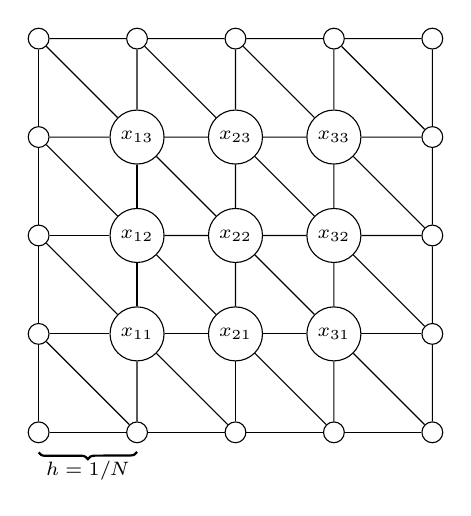
\begin{tikzpicture}[scale=5]

	\scriptsize
	% Place each of the nodes in the grid
    % First the boundary nodes
    \foreach \x in {0,...,4}
    	\foreach \y in {0,4}
    {
    	\node[circle,draw=black]
          (\x\y) at (0.25*\x,0.25*\y) {};
    }
    
    \foreach \y in {1,...,3}
        \foreach \x in {0, 4}
    {
    	\node[circle,draw=black]
          (\x\y) at (0.25*\x,0.25*\y) {};
    }
    
    % Now the interior nodes - plus labels
   	\foreach \x in {1,...,3}
		\foreach \y in {1,...,3}
    {
         \node[circle,draw=black] 
            (\x\y) at (0.25*\x,0.25*\y) {$x_{\x\y}$};
    }
    
    % Next, the horizontal grid lines
    \foreach \y in {0,...,4}
       \foreach \x in {0,...,3}
    {
    	\pgfmathtruncatemacro{\idx}{\x + 1}
        \draw (\x\y) -- (\idx\y);
    }
    
    % Now for the verticals
    \foreach \x in {0,...,4}
        \foreach \y in {0,...,3}
    {
    	\pgfmathtruncatemacro{\idx}{\y + 1}
        \draw(\x\y) -- (\x\idx);
    }
    
    % Finally... the diagonals
    \foreach \y in {1,...,4}
        \foreach \x in {0,...,3}
    {
    	\pgfmathtruncatemacro{\xidx}{\x + 1}
        \pgfmathtruncatemacro{\yidx}{\y - 1}
        \draw (\x\y) -- (\xidx\yidx);
    }
    
    % Bonus round, show the density of the grid
    \draw[thick,decoration={brace,mirror},decorate]
      (0,-0.051) -- (0.25, -0.05)
      node[pos=0.5,anchor=north]{$h=1/N$};
\end{tikzpicture}
\caption{Example triangulation of $\Omega$ with $N = 4$}
\label{fig:two-d-discretisation}
\end{figure}

Using this triangulation we can now define suitable finite dimensional subspaces
of our test and trial spaces $V^h \subset V$, $W^h \subset W$:

\begin{align*}
	V^h = \{v \in V: &v \text{ is linear on } T_k,\ k \in \{1,\ldots,2N^2\}, \\
                     &v \text{ is continuous on } \Omega\}
\end{align*}

Then by choosing appropriate basis functions $\phi_i$ for the above subspaces we will be able to approximate
the solution as follows:

\begin{equation}
	u^h(\v{x}) = \sum_{j=1}^{(N+1)^2}u_j\phi_j(\v{x})
\end{equation}

where $u_j$ will be the approximate value of the solution at the node $x_j$. Similarly we can
approximate $f(\v{x})$:

\begin{equation}
	f(x) \approx \sum_{j=1}^{(N+1)^2}f_j\phi_j(\v{x})
\end{equation}

where $f_j = f(\v{x_j})$

\todo[inline]{Give details on errors, convergence etc!}

As in the one dimensional case, an appropriate basis would be the `hat functions' which we can define in
terms of a reference function $\Phi(\v{x})$ defined with respect to an example domain around $(0,0)$.
Consider as in Figure \ref{fig:reference-function-domain} the domain where the function has support, 
then we can write $\Phi(\v{x})$ as follows:

\begin{equation}\label{eq:two-d-ref-basis-fn}
	\Phi(\v{x}) = \left\{\begin{array}{c c}
					1 - \frac{(x + y)}{h}, & \text{ in } T_1 \\
                    1 - \frac{x}{y},       & \text{ in } T_2 \\
                    1 + \frac{y}{h},       & \text{ in } T_3 \\
                    1 + \frac{(x + y)}{h}, & \text{ in } T_4 \\
                    1 + \frac{x}{h},       & \text{ in } T_5 \\
                    1 - \frac{y}{h},       & \text{ in } T_6 \\
                    0,                     & \text{ otherwise}
 	              \end{array}\right.
\end{equation}

where $\v{x} = (x, y)$. Then we can write each basis function $\phi_i$ in our discretised domain as
$\phi_i(\v{x}) = \Phi(\v{x_i} - \v{x})$

\begin{figure}
\centering
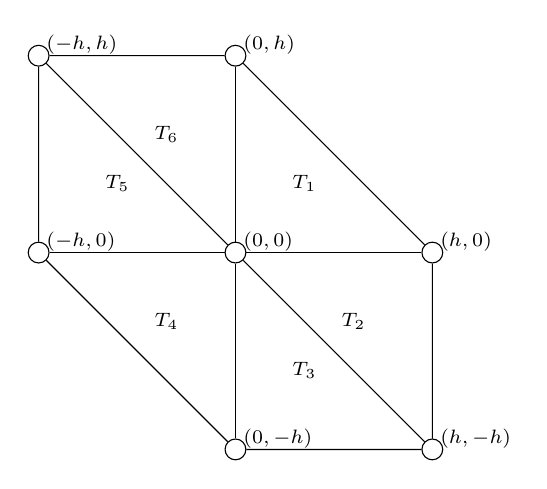
\begin{tikzpicture}[scale=2.5]
	\scriptsize
    
    % Place the nodes
    \node[circle,draw=black,label={[anchor=west]$(0,0)$}] (00)  at (0,0)  {};
    \node[circle,draw=black,label={[anchor=west]$(0,h)$}] (01)  at (0,1) {};
    \node[circle,draw=black,label={[anchor=west]$(h,0)$}] (10)  at (1,0)  {};
    \node[circle,draw=black,label={[anchor=west]$(-h,0)$}] (-10) at (-1,0) {};
    \node[circle,draw=black,label={[anchor=west]$(0,-h)$}] (0-1) at (0,-1) {};
    \node[circle,draw=black,label={[anchor=west]$(-h,h)$}] (-11) at (-1,1) {};
    \node[circle,draw=black,label={[anchor=west]$(h,-h)$}] (1-1) at (1,-1) {};
    
    % Draw the lines
    \draw (00) -- (01);
    \draw (00) -- (10);
    \draw (01) -- (10);
    \draw (00) -- (-10);
    \draw (00) -- (0-1);
    \draw (-11) -- (01);
    \draw (-11) -- (00);
    \draw (-11) -- (-10);
    \draw (-10) -- (0-1);
    \draw (0-1) -- (1-1);
    \draw (1-1) -- (10);
    \draw (00) -- (1-1);
    
    % Finally the T's
    \node (T1) at (0.35,0.35) {$T_1$};
    \node (T2) at (0.6, -0.35) {$T_2$};
    \node (T3) at (0.35, -0.6) {$T_3$};
    \node (T4) at (-0.35,-0.35) {$T_4$};
    \node (T5) at (-0.6, 0.35) {$T_5$};
    \node (T6) at (-0.35, 0.6) {$T_6$};
  
\end{tikzpicture}
\caption{The domain of the reference function $\Phi(\v{x})$}
\label{fig:reference-function-domain}
\end{figure}

As we will see it will be useful to introduce a mapping that will let us
evaluate integrals for arbitrary triangles by considering a single reference
triangle comprised of the points $(0,0), (0,1), (1,0)$

\todo[inline]{Explain the master triangle, the mapping etc}

\begin{align}\label{eq:master_basis_functions}
    \psi_1(\zeta, \eta) &= 1 - \zeta - \eta \\
    \psi_2(\zeta, \eta) &= \zeta \\
    \psi_3(\zeta, \eta) &= \eta
\end{align}

It will also be useful to consider the derivatives of these functions:

\begin{align}\label{eq:master_basis_functions_derivative}
    \psi_1' = \nabla\psi_1(\zeta, \eta) &=
        \frac{1}{h}\left(\begin{array}{c}-1 \\ -1\end{array}\right) \\
    \psi_2' = \nabla\psi_2(\zeta, \eta) &=
        \frac{1}{h}\left(\begin{array}{c}1 \\ 0\end{array}\right) \\
    \psi_3' = \nabla\psi_3(\zeta, \eta) &=
        \frac{1}{h}\left(\begin{array}{c}0 \\ 1\end{array}\right)
\end{align}

\section{The Local Stiffness Matrix}

Each local stiffness matrix will have dimension $3 \times 3$ and will be given
by:

\begin{align*}
    A^k_{i,j} &= a_k(\phi_j, \phi_i) \\
     &= \int_{T_k}a\nabla\phi_i\cdot\nabla\phi_j\,dxdy +
        \int_{T_k}\v{b}\cdot\phi_j\nabla\phi_i\,dxdy +
        \int_{T_k}c\phi_i\phi_j\,dxdy
\end{align*}

To simplify the integrations we will apply our mapping so that we have:

\[
    A^k_{i,j} = h^2\int_Ta\nabla\psi_i\cdot\nabla\psi_j\,d\zeta d\eta +
                h^2\int_T\v{b}\psi_j\nabla\psi_i\,d\zeta d\eta +
                h^2\int_Tc\psi_i\psi_j\,d\zeta d\eta
\]

Considering each term in isolation:

\[
    ah^2\int_T\nabla\psi_i\cdot\nabla\psi_j\,d\zeta d\eta =
    a\int_T\psi'_{i\zeta}\psi'_{j\zeta} +
        \psi'_{i\eta}\psi'_{i\eta}\,d\zeta d\eta
\]

We can see from this that the resulting matrix will be symmetric, let's
consider the case when $i = 1 = j$:

\begin{align*}
    a\int_T(\psi'_{1\zeta})^2 + (\psi'_{1\eta})^2\,d\zeta d\eta & =
        a\int_T(-1)^2 + (-1)^2\,d\zeta d\eta \\
    &= 2a\int_0^1\int_0^\eta\,d\zeta d\eta \\
    &= 2a\frac{1}{2} \\
    &= a
\end{align*}

Evaluating similar integrals for each entry in the matrix results in the following
local stiffness matrix associated with the Laplacian term:

\begin{equation}\label{eq:stiffness_term_1}
    a\left(\begin{array}{c c c}
        1      & -\half & -\half \\
        -\half & \half  & 0 \\
        -\half & 0      & \half
    \end{array}\right)
\end{equation}

Now let's consider the second term, in the case when $i = 2, j = 1$:

\begin{align*}
    h^2\int_T{\v{b}\psi_1\nabla\psi_2}\, d\zeta d\eta &=
    -h\int_0^1\int_0^\eta{\zeta b_x + \zeta b_y}\, d\zeta d\eta \\
    &= -h(b_x + b_y)\int_0^1\int_0^\eta{\zeta}\, d\zeta d\eta \\
    &= -\frac{h(b_x + b_y)}{6}
\end{align*}

Repeating this for the other entries we get the matrix:

\begin{equation}\label{eq:stiffness_term_2}
    h\left(\begin{array}{c c c}
        -\frac{(b_x + b_y)}{12} & \frac{b_x}{6} & \frac{b_y}{6} \\
        -\frac{(b_x + b_y)}{12} & \frac{b_x}{6} & \frac{b_y}{6} \\
        -\frac{(b_x + b_y)}{12} & \frac{b_x}{6} & \frac{b_y}{6}
    \end{array}\right)
\end{equation}

Finally let's consider the third integral, in the case where $i = j = 1$:

\begin{align*}
       ch^2\int_T{\psi_1\psi_1}\,d\zeta d\eta
       &= ch^2\int_0^1\int_0^\eta{(1 - \zeta - \eta)^2}\, d\zeta d\eta \\
%
       &= ch^2\int_0^1\int_0^\eta\, d\zeta d\eta +
          2ch^2\int_0^1\int_0^\eta{\zeta\eta - \zeta - \eta}\, d\zeta d\eta +
          ch^2\int_0^1\int_0^\eta{\zeta^2 + \eta^2}\, d\zeta d\eta \\
%
       &= \frac{ch^2}{2} - \frac{3ch^2}{4} + \frac{ch^2}{3} \\
       &= \frac{ch^2}{12}
\end{align*}

Following a similar argument for the other entries gives us the following
matrix:

\begin{equation}\label{eq:stiffness_term_3}
    \frac{ch^2}{2}\left(\begin{array}{c c c}
         \frac{1}{12} &  \frac{1}{24} &  \frac{1}{24} \\
         \frac{1}{24} &  \frac{1}{12} &  \frac{1}{24} \\
         \frac{1}{24} &  \frac{1}{24} &  \frac{1}{12}
    \end{array}\right)
\end{equation}

Combining (\ref{eq:stiffness_term_1}), (\ref{eq:stiffness_term_2}),
(\ref{eq:stiffness_term_3}) gives us the local stiffness matrix for the general
form of the equation (\ref{eq:general_laplace})

\section{The Local Mass Matrix}

The local mass matrix will also have dimension $3 \times 3$

    \include{chapters/chapter2}
    \include{chapters/chapter3}

    % The bibliography:
    \printbibliography
\end{document}
